%! TeX program = lualatex
% - - - - - - - - - - - - - - - - - - - - - - - - - - - - - - - - - - - - - - - 
% Core setup
% - - - - - - - - - - - - - - - - - - - - - - - - - - - - - - - - - - - - - - - 
\documentclass[10pt,a4paper]{article}
%\documentclass[10pt,a4paper,article,oneside]{memoir}
\usepackage[top=2.5cm,right=2.5cm,bottom=2.5cm,left=2.5cm,footnotesep=1cm]{geometry}
\usepackage{etoolbox}             % If statements and boolean values
\usepackage[norsk]{babel}         % Support for other languages than english
\usepackage[utf8]{inputenc}       % Input encoding
\usepackage[T1]{fontenc}          % Font encoding
\usepackage{microtype}            % Improve text appearance in numerous ways
\usepackage{textcomp}             % Add extra symbols
\usepackage{mathtools}            % Improvements for math
\usepackage{amssymb}              % Extended math symbols


% - - - - - - - - - - - - - - - - - - - - - - - - - - - - - - - - - - - - - - - 
% Font packages
% - - - - - - - - - - - - - - - - - - - - - - - - - - - - - - - - - - - - - - - 
%\usepackage[osf]{newpxtext}       % Main (serif/sans-serif) font
\usepackage[nomath,nott,noamsmath,notextcomp,oldstylenums,light]{kpfonts} % Main (serif/sans-serif) font
\usepackage{newpxmath}            % Math font
\usepackage[scaled]{beramono}     % Monospace font
\usepackage{iftex}
\ifLuaTeX
    \usepackage{fontspec}                % Custom fonts
    \setmonofont{PxPlus ToshibaSat 8x16} % Override monospace font
\fi


% - - - - - - - - - - - - - - - - - - - - - - - - - - - - - - - - - - - - - - - 
% Additional packages
% - - - - - - - - - - - - - - - - - - - - - - - - - - - - - - - - - - - - - - - 
\usepackage[T1]{url}\urlstyle{sf} % Clickable URLs
\usepackage{hyperref}             % Clickable references
\usepackage{csquotes}             % Support quote marks in various languages
\usepackage{caption}              % Caption customization
\usepackage{ulem}                 % Double underline
\usepackage[makeroom]{cancel}     % Crossing out text
\usepackage{nicefrac}             % Nice looking fractals
\usepackage[compact]{titlesec}    % Title style
\usepackage{setspace}             % Set paragraph spacing
\usepackage{xcolor}               % Colors
\usepackage{enumitem}             % Lists
\usepackage{listings}             % Insert code
\usepackage{tikz}                 % Drawing of graphics
\usepackage{graphicx}             % Insert images
\usepackage{booktabs}             % Nicer looking tables
\usepackage{fancyhdr}             % Header / footer
\usepackage{lastpage}             % Last page number
\usepackage{marginnote}           % Margin notes
%\usepackage{pdfpages}             % Insert pdf pages
%\usepackage{biblatex}             % Bibliography
%\usepackage{gensymb}              % Degree symbol
%\usepackage{verbatim}             % Comments
%\usepackage{units}
%\usapackage{siunitx}
%\usepackage{cleverref}

% - - - - - - - - - - - - - - - - - - - - - - - - - - - - - - - - - - - - - - - 
% Apprentice colorscheme (https://github.com/romainl/Apprentice)
% - - - - - - - - - - - - - - - - - - - - - - - - - - - - - - - - - - - - - - - 
\definecolor{color0}{HTML}{1C1C1C}
\definecolor{color1}{HTML}{AF5F5F}
\definecolor{color2}{HTML}{5F875F}
\definecolor{color3}{HTML}{87875F}
\definecolor{color4}{HTML}{5F87AF}
\definecolor{color5}{HTML}{5F5F87}
\definecolor{color6}{HTML}{5F8787}
\definecolor{color7}{HTML}{6C6C6C}
\definecolor{color8}{HTML}{444444}
\definecolor{color9}{HTML}{FF8700}
\definecolor{color10}{HTML}{87AF87}
\definecolor{color11}{HTML}{FFFFAF}
\definecolor{color12}{HTML}{87AFD7}
\definecolor{color13}{HTML}{8787AF}
\definecolor{color14}{HTML}{5FAFAF}
\definecolor{color15}{HTML}{FFFFFF}
\definecolor{colorfg}{HTML}{BCBCBC}
\definecolor{colorbg}{HTML}{262626}


% - - - - - - - - - - - - - - - - - - - - - - - - - - - - - - - - - - - - - - - 
% Habamax colorscheme (https://github.com/habamax/vim-habamax)
% - - - - - - - - - - - - - - - - - - - - - - - - - - - - - - - - - - - - - - - 
\definecolor{brightCyan}{HTML}{87AFAF}
\definecolor{cyan}{HTML}{5F8787}
\definecolor{darkCyan}{HTML}{1F3F5F}
\definecolor{pink}{HTML}{D75F87}
\definecolor{red}{HTML}{D75F5F}
\definecolor{darkRed}{HTML}{AF5F5F}
\definecolor{brightGreen}{HTML}{5FF75F}
\definecolor{green}{HTML}{87D787}
\definecolor{darkGreen}{HTML}{5FAF5F}
\definecolor{blue}{HTML}{5fafd7}
\definecolor{darkBlue}{HTML}{5F87AF}
\definecolor{brightYellow}{HTML}{ffaf5f}
\definecolor{yellow}{HTML}{d7af87}
\definecolor{darkYellow}{HTML}{af875f}
\definecolor{brightMagenta}{HTML}{ff00af}
\definecolor{magenta}{HTML}{d787d7}
\definecolor{darkMagenta}{HTML}{af87af}


% - - - - - - - - - - - - - - - - - - - - - - - - - - - - - - - - - - - - - - - 
% Custom commands
% - - - - - - - - - - - - - - - - - - - - - - - - - - - - - - - - - - - - - - - 
%\usepackage{soul}                 % Character spacing
%\sodef\allcapsspacing{\upshape}{0.15em}{0.65em}{0.6em}
%\sodef\lowsmallcapsspacing{\scshape}{0.075em}{0.5em}{0.6em}
%\newcommand{\allcaps}[1]{\MakeUppercase{\allcapsspacing{#1}}}%   
%\newcommand{\smallcaps}[1]{\MakeLowercase{\textsc{\lowsmallcapsspacing{#1}}}}
\newcommand{\oppgave}[1]{\subsection*{Oppgave #1}}
\newcommand{\oppgaveDelStart}{\begin{enumerate}[leftmargin=*,itemsep=1.5cm,labelsep=1.5em,label=\alph*)]}
\newcommand{\oppgaveDelSlutt}{\end{enumerate}}
\newcommand{\oppgaveDel}[1]{\item[\textbf{#1})]}
\newcommand\N{\ensuremath{\mathbb{N}}}
\newcommand\R{\ensuremath{\mathbb{R}}}
\newcommand\Z{\ensuremath{\mathbb{Z}}}
\newcommand\Q{\ensuremath{\mathbb{Q}}}
\newcommand\C{\ensuremath{\mathbb{C}}}
\newcommand{\threestars}{\begin{center}\par * * * \end{center}}


% - - - - - - - - - - - - - - - - - - - - - - - - - - - - - - - - - - - - - - - 
% Package settings
% - - - - - - - - - - - - - - - - - - - - - - - - - - - - - - - - - - - - - - - 
\providetoggle{margin}
\settoggle{margin}{true}
\iftoggle{margin}{
    \geometry{right=5cm, marginparsep=0.8cm, marginparwidth=3.4cm}
    \lstset{xrightmargin=-2.5cm}
}{}
\renewcommand*{\marginfont}{\footnotesize}
\pagestyle{fancy}\fancyhf{}
\fancyhead[L]{\normalsize\scshape\MakeLowercase{\emne \ \ \textendash \ \ \tittel}}
\fancyfoot[C]{\normalsize{\thepage} \scriptsize{/} \normalsize{\pageref{LastPage}}}
\fancypagestyle{first}{\fancyhead[L,C,R]{}\renewcommand{\headrulewidth}{0pt}}
\hypersetup{colorlinks=true, urlcolor=pink, filecolor=pink, linkcolor=color0, citecolor=color0, anchorcolor=color0}
\captionsetup{format=hang, font=footnotesize, labelfont=bf, labelsep=endash, labelformat=empty}
\captionsetup{width=0.8\textwidth}
\usetikzlibrary{shapes.multipart, shadows, positioning, calc}
\color{color0}
\linespread{1.05}
\setlength{\parindent}{0pt}
%\setlength{\tabcolsep}{18pt}
%\renewcommand{\arraystretch}{1.25}
\newlength{\myeqskip}\setlength{\myeqskip}{2pt}
\titlespacing*{\section}{0cm}{0.8ex}{1.2ex}
\titleformat{\section}{\normalfont\large\bfseries\scshape\MakeLowercase}{\thesection \ \ \textendash \ \ }{0em}{}
\titleformat{\subsection}{\normalfont\normalsize\bfseries}{\thesubsection.}{0.75em}{}
\titleformat{\subsubsection}{\normalfont\normalsize\itshape}{\thesubsubsection.}{0.75em}{}
\lstset{literate={æ}{{\ae}}1{Æ}{{\AE}}1{ø}{{\o}}1{Ø}{{\O}}1{å}{{\aa}}1{Å}{{\AA}}1,
keywordstyle={\bfseries\color{color1}}, 
commentstyle={\bfseries\color{cyan}},
basicstyle={\scriptsize\ttfamily\color{color0}}, 
numbers=none,numberstyle={\scriptsize\ttfamily\color{color7}},
aboveskip=0.1cm,belowskip=1cm,columns=fixed,
breaklines=true,breakatwhitespace=false,keepspaces=true,
showspaces=false,showstringspaces=false,tabsize=4,
captionpos=b,inputencoding=utf8,extendedchars=true}


% - - - - - - - - - - - - - - - - - - - - - - - - - - - - - - - - - - - - - - - 
% Set course / title / author
% - - - - - - - - - - - - - - - - - - - - - - - - - - - - - - - - - - - - - - - 
\newcommand{\emne}{DAT102}
\newcommand{\tittel}{Obligatorisk innlevering 1}
\newcommand{\gruppemedlemmer}{Stephen Neba Fuh, \ Tord Johan Melheim, \\ Ebubekir Siddik Yuksel, \ Casper Eide Özdemir-Børretzen}


% - - - - - - - - - - - - - - - - - - - - - - - - - - - - - - - - - - - - - - - 
% Document start and title page
% - - - - - - - - - - - - - - - - - - - - - - - - - - - - - - - - - - - - - - - 
\begin{document}
%\begin{titlepage}
\thispagestyle{first}
\vspace*{0.8cm}
\par\includegraphics[scale=0.035]{hvl.png}
\vspace{0.15cm}
\par\normalsize{Institutt for datateknologi, elektroteknologi og realfag}
\vspace{0.30cm}
\hrule
\vspace{0.30cm}
\par\Large\textbf{\emne \ \ $\mid$ \ \ \tittel}
\vspace{0.25cm}
\hrule
\vspace{0.35cm}
%\par\footnotesize{Gruppemedlemmer:}
%\vspace{0.1cm}
\par\normalsize\textbf{\gruppemedlemmer}
\par\footnotesize{22. februar 2026}
\vspace*{2cm}
%\end{titlepage}
\normalsize


% - - - - - - - - - - - - - - - - - - - - - - - - - - - - - - - - - - - - - - - 
% Main content
% - - - - - - - - - - - - - - - - - - - - - - - - - - - - - - - - - - - - - - - 
% Dummy text taken from the LaTeX lipsum package

\section{Pellentesque dolor felis}

Lorem ipsum dolor sit amet,
consectetuer adipiscing elit
\footnote{Aliquam tempus ipsum urna, sit amet hendrerit neque tempor vel. Integer eu urna euismod, euismod odio sit amet, fermentum dolor. \url{https://ctan.org/pkg/lipsum}}
\mnFig{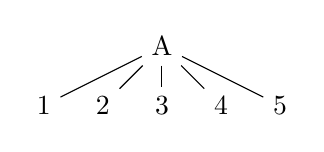
\begin{tikzpicture}[scale=0.5]
\node {A}
child { node {1} }
child { node {2} }
child { node {3} }
child { node {4} }
child { node {5} }
;
\end{tikzpicture}}
{Mauris pulvinar placerat varius. Ut eu semper nulla, eu pharetra ex.}
. Ut purus elit, vestibulum ut, placerat ac, adipiscing vitae, felis. Curabitur dictum gravida mauris. Nam arcu libero, nonummy eget, consectetuer id, vulputate a, magna. Donec vehicula augue eu neque. 
Pellentesque habitant morbi tristique senectus et netus et malesuada fames ac turpis egestas. Mauris ut leo. Cras viverra metus rhoncus sem. Nulla et lectus vestibulum urna fringilla ultrices.  Phasellus eu tellus sit amet tortor gravida placerat.
Integer sapien est, iaculis in, pretium quis, viverra ac, nunc. Praesent eget sem vel leo ultrices bibendum. Aenean faucibus. Morbi dolor nulla, malesuada eu, pulvinar at, mollis ac, nulla. %Curabitur auctor semper nulla. Donec varius orci eget risus. Duis nibh mi, congue eu, accumsan eleifend, sagittis quis, diam. Duis eget orci sit amet orci dignissim rutrum.

\vspace{1cm}

\begin{center}
\begin{tabular}{lcccccl}\toprule
& \multicolumn{3}{c}{$abc$} & \multicolumn{3}{c}{$def$}
\\\cmidrule(lr){2-4}\cmidrule(lr){5-7}
         & $mv$   & Rel.~err & Time  & $mv$    & Rel.~err & Time\\\midrule
a        & 11034  & 1.3e-7   & 3.9   & 15846   & 2.7e-11  & 5.6 \\
b        & 21952  & 1.3e-7   & 6.2   & 31516   & 2.7e-11  & 8.8 \\
c        & 15883  & 5.2e-8   & 7.1   & 32023   & 1.1e-11  & 1.4e1\\\bottomrule
\end{tabular}
\end{center}

\vspace{1cm}

\subsection{Morbi vel justo vitae lacus tincidunt ultrices}

Nam dui ligula, 
\mn{Maecenas semper, magna in suscipit maximus, diam libero ultricies neque, eget placerat elit ante ut diam. Aenean a lacus at elit venenatis iaculis sit amet non est. Nam vel ullamcorper nisi. Vivamus lacinia quis quam quis posuere. Proin vel posuere lacus, eu rhoncus tortor. Nullam vel felis quis massa lacinia laoreet. Sed eget lacinia tellus.}
fringilla a, euismod sodales, sollicitudin vel, wisi. Morbi auctor lorem non justo. Nam lacus libero, pretium at, lobortis vitae, ultricies et, tellus:

\begin{enumerate}
\item In hac habitasse platea dictumst;
\item In hac habitasse platea dictumst;
\item Nunc elementum fermentum wisi.
\end{enumerate}

\noindent\textit{Donec aliquet, tortor sed accumsan bibendum, erat ligula aliquet magna, vitae ornare odio metus a mi. Morbi ac orci et nisl hendrerit mollis. Suspendisse ut massa. Cras nec ante. Pellentesque a nulla. Cum sociis natoque penatibus et magnis dis parturient montes, nascetur ridiculus mus.} % Aliquam tincidunt urna. Nulla ullamcorper vestibulum turpis. Pellentesque cursus luctus mauris.}

\newpage

\section{Sample page of source code}

%\begin{fullwidth}
\begin{lstlisting}[language=Java]
private static int s(int n) {
    return n == 1 ? 1 : s(n-1) + n;
}

private static int sAntKall(int n) {
    return n == 1 ? 1 : sAntKall(n-1) + 1;
}

public static void main(String[] args) {
    System.out.printf("S_n = S_{n-1} + n, S_1 = 1%nS_{100} = %d%nS_{100} gjennomfører %d kall på s(n) funksjonen.%nn = 100 -> 100 funksjonskall.%nDette kan uttrykkes som O(n) i O-notasjon.%n", s(100), sAntKall(100));
}

/*
Dette gir resultatet:
    S_n = S_{n-1} + n, S_1 = 1
    S_{100} = 5050
    S_{100} gjennomfører 100 kall på s(n) funksjonen.
    n = 100 -> 100 funksjonskall.
    Dette kan uttrykkes som O(n) i O-notasjon.
*/
\end{lstlisting}
%\end{fullwidth}

\vspace*{20pt}

\newcommand{\abc}{abcdefghijklmnopqrstuvwxyz}
\newcommand{\ABC}{ABCDEFGHIJKLMNOPQRSTUVWXYZ}
\newcommand{\alphabeta}{\alpha\beta\gamma\delta\epsilon\varepsilon\zeta\eta\theta\vartheta\iota\kappa\varkappa\lambda\mu\nu\xi o\pi\varpi\rho\varrho\sigma\varsigma\tau\upsilon\phi\varphi\chi\psi\omega}
\newcommand{\AlphaBeta}{\Gamma\Delta\Theta\Lambda\Xi\Pi\Sigma\Upsilon\Phi\Psi\Omega}

\small

\noindent$01234567890$

\noindent$\abc$

\noindent$\ABC$

\noindent$\alphabeta$

\noindent$\AlphaBeta$

\noindent$\ell\wp\aleph\infty\propto\emptyset\nabla\partial\mho\imath\jmath\hslash\eth$

\noindent$\mathrm{A} \Lambda \Delta \nabla \mathrm{B C D} \Sigma \mathrm{E F} \Gamma \mathrm{G H I J K L M N O} \Theta \Omega \mho \mathrm{P} \Phi \Pi \Xi \mathrm{Q R S T U V W X Y} \Upsilon \Psi \mathrm{Z} $ % $ \quad 1234567890 $

\noindent$\mathit{A \Lambda \Delta B C D E F \Gamma G H I J K L M N O \Theta \Omega P \Phi \Pi \Xi Q R S T U V W X Y \Upsilon \Psi Z }$

% don't allow overfull boxes
% {\par \tolerance=0 \emergencystretch=100em $a\alpha b \beta c \partial d \delta e \epsilon \varepsilon f \zeta \xi g \gamma h \hbar \hslash \iota i \imath j \jmath k \kappa \varkappa l \ell \lambda m n \eta \theta \vartheta o \sigma \varsigma \phi \varphi \wp p \rho \varrho q r s t \tau \pi u \mu \nu v \upsilon w \omega \varpi x \chi y \psi z$ \linebreak[3] $\infty \propto \emptyset \varnothing \mathrm{d}\eth \backepsilon$\par}
%\noindent$\mathbb{\ABC}$
%\noindent$\mathcal{\ABC}$
%\noindent$\bm{\ABC}$

\newpage

% The first maths sample is taken from Example 8-8-10 of The LaTeX Companion

\section{Sample page of mathematical typesetting}

First some large operators
both in text: \( \iiint\limits_{\mathcal{Q}}
f(x,y,z)\,dx\,dy\,dz \) and
\(\prod_{\gamma\in\Gamma_{\widetilde{C}}}
\partial(\widetilde{X}_\gamma)\); and also on display:

For $x$ in the open interval \( \left] -1, 1 \right[ \)
the infinite sum in Equation~\eqref{eq:binom1} is convergent;
however, this does not hold
throughout the closed interval \( \left[ -1, 1 \right] \).
\begin{align}
  (1 - x)^{-k} &=
    1 + \sum_{j=1}^{\infty} (-1)^j \genfrac\lbrace\rbrace{0pt}{}{k}{j} x^j
    \text{\quad for $k \in \mathbb{N}$; $k \neq 0$.}
    \label{eq:binom1}
\end{align}


% The second maths sample is taken from the article "A Survey of Free Math Fonts for TeX and LaTeX" by Stephen G. Hartke

\noindent\textbf{Theorem 1 (Residue Theorem).}
Let $f$ be analytic in the region $G$ except for the isolated singularities $a_1,a_2,\ldots,a_m$. If $\gamma$ is a closed rectifiable curve in $G$ which does not pass through any of the points $a_k$ and if $\gamma\approx 0$ in $G$ then
\[
\frac{1}{2\pi i}\int_\gamma f = \sum_{k=1}^m n(\gamma;a_k) \text{Res}(f;a_k).
\]

\noindent\textbf{Theorem 2 (Maximum Modulus).}
\emph{Let $G$ be a bounded open set in $\mathbb{C}$ and suppose that $f$ is a continuous function on $G^-$ which is analytic in $G$. Then}
\[
\max\{|f(z)|:z\in G^-\}=\max \{|f(z)|:z\in \partial G \}.
\]




% - - - - - - - - - - - - - - - - - - - - - - - - - - - - - - - - - - - - - - - 

\end{document}
